% This is the LaTex style file for HCLT 2026, 
% modified version of the style used for ACL and NIPS.
% If you are an Overleaf user, please edit "Menu->TeX Live version-> 2021".
% --  Chanjun Park, Cheoneum Park

\documentclass[twocolumn, 10pt]{article}

\usepackage{hclt}
\usepackage[utf8]{inputenc}
\usepackage[pdfencoding=auto]{hyperref}
\usepackage{url}
\usepackage{amsmath}
\usepackage{latexsym}
\usepackage{amssymb}
\usepackage{graphicx}

\DeclareMathOperator*{\argmax}{arg\,max}
\DeclareMathOperator*{\argmin}{arg\,min}

\title[korean]{국문 제목}
\title[english]{English Title}

\author[korean]{
홍길동$^{\circ}$, 김길수 \\
한국대학 한국학부\\
\texttt{\{hong,kim\}@mail.ac.kr}\\
}

\author[english]{
Gil-Dong Hong$^{\circ}$, Gil-Su Kim \\
Hanguk University, Hanguk Research Institute
}

% \finalcopy % Uncomment for camera-ready version

\begin{document}

\twocolumn[
\maketitle
\begin{abstract}
이 부분은 학술 논문의 요약(Abstract)을 작성하는 영역입니다. 연구의 목적, 방법, 주요 결과, 의의 등을 간결하고 명확하게 서술해야 하며, 전체 논문의 핵심 내용을 함축적으로 전달해야 합니다.
\end{abstract}

\begin{keyword}
초거대언어모델, 기계번역, 정보검색
\end{keyword}
]

\section{서론}
이 문서는 한글 및 한국어 정보처리 학술대회 tex 양식을 설명한 문서입니다.
기본 파일은 3개입니다.
한글 및 한국어 정보처리 학술대회의 논문 양식에 대한 스타일 파일 `hclt.sty',
참고문헌 서식에 대해 정의한 `IEEEtran.bst' 및
논문 내용을 작성하는 `hclt.tex' 파일입니다.
%로 구성되어 있습니다.
그 외, 참고문헌을 위한 bibtex 파일인 `refer.bib', 그림 `cat.jpg, neuron.jpg' 파일들이 tex 작성 방법을 설명하기 위해 첨부되어 있습니다.

이 파일은 한글 파일 양식에 기술된 구성을 똑같이 따르고 있습니다.
Tex으로 논문을 작성하면 미려한 논문을 작성할 수 있는 장점을 가지고 있습니다.

\section{학술대회 논문작성 시 유의사항}
논문 페이지 수는 2쪽 이상 6쪽 이내입니다. 단, 구두발표는 3페이지 이상 작성하셔야 합니다. 본 tex 파일의 용지 및 여백 처리, 논문 구성은 제31회 한글 및 한국어 정보처리 학술대회에서 사용하고 있는 한글 파일 양식에 기술된 내용을 따르고 있습니다.

한글 및 한국어 정보처리 학술대회는 암행평가(blind review)로 논문을 평가합니다.
따라서, 심사용 논문에는 저자정보(이름, 소속, 이메일)를 일절 표기하지 않습니다.
본 tex파일은 저자 정보를 입력할지라도 기본 저자 정보(이름, 소속, 이메일, Anonymous Author(s), Affiliation)로 논문을 생성합니다.
최종본을 제출시, 문서 상단의 \textbackslash{finalcopy}을 주석해제하여 저자 정보가 있는 논문을 생성할 수 있습니다.
발표자는 공동저자와 구분 처리해야 하는 규정에 따라 \textbackslash{circ}~을 사용하여 표기하고 있습니다.
장, 절, 조에 대해서는 각각 \textbackslash{section}, \textbackslash{subsection}, \textbackslash{subsubsection}\을 사용하시면 됩니다.

\subsection{글머리표 작성법}
숫자가 없는 글머리표에 대해서는 \textbackslash{itemize}\를 사용하여 작성할 수 있습니다.
\begin{itemize}
\item 용지: A4, 가로쓰기
\item 위쪽 여백: 30mm
\item 아래쪽 여백: 20mm
\item 왼쪽 여백: 10mm
\item 오른쪽 여백: 10mm
\end{itemize}
예제에서 보는 것과 같이 \textbackslash{item}\을 추가하여 항목을 늘릴 수가 있습니다.

숫자가 있는 글머리표는 \textbackslash{enumerate}\를 사용하면 됩니다.
\begin{enumerate}
  \item 숫자 글머리표 1
  \item 숫자 글머리표 2
  \item 숫자 글머리표 3
\end{enumerate}

글머리표 작성은 \url{https://www.overleaf.com/learn/latex/Lists}에서 자세히 살펴볼 수 있습니다.

\subsection{수식 작성법}
Tex에서는 가독성이 좋은 수식을 작성할 수 있습니다.
예시를 위해 Support Vector Machine (SVM)의 최적화 수식을 설명합니다~\cite{crammer:jmlr2002}.
편의상 변수에 대한 설명은 생략합니다.
\begin{eqnarray}
\underset{w,\xi}{\min}\frac{1}{2}||w||^2 + C\sum_{i=1}^{l}\xi_i, \label{eqn:svm}
\end{eqnarray}
subject to
\begin{eqnarray}
y_i(x_i \cdot w + b) \ge 1 - \xi_i, \text{ and } \xi_i \ge 0 ~~\forall i.\nonumber
\end{eqnarray}
수식 \eqref{eqn:svm}\와 달리 \textbackslash{nonumber}\을 통해 제약조건 나타낸 수식에는 참조 번호를 부착하지 않을 수도 있습니다.
수식 작성은 \url{https://en.wikibooks.org/wiki/LaTeX/Mathematics}에서 자세히 살펴볼 수 있습니다.

\subsection{그림/표 작성법}
\begin{table}[t]
\caption{세종 데이터 셋의 통계정보}
\label{tab:data_stats}
\begin{center}
\begin{tabular}{c|c|c}
\hline
 & 학습 데이터 & 평가 데이터 \\
\hline
단어 수   & 1,234 & 2,345 \\
문장 수   & 5,555 & 6,666 \\
\hline
\end{tabular}
\end{center}
\end{table}

\begin{figure}[t]
\centering
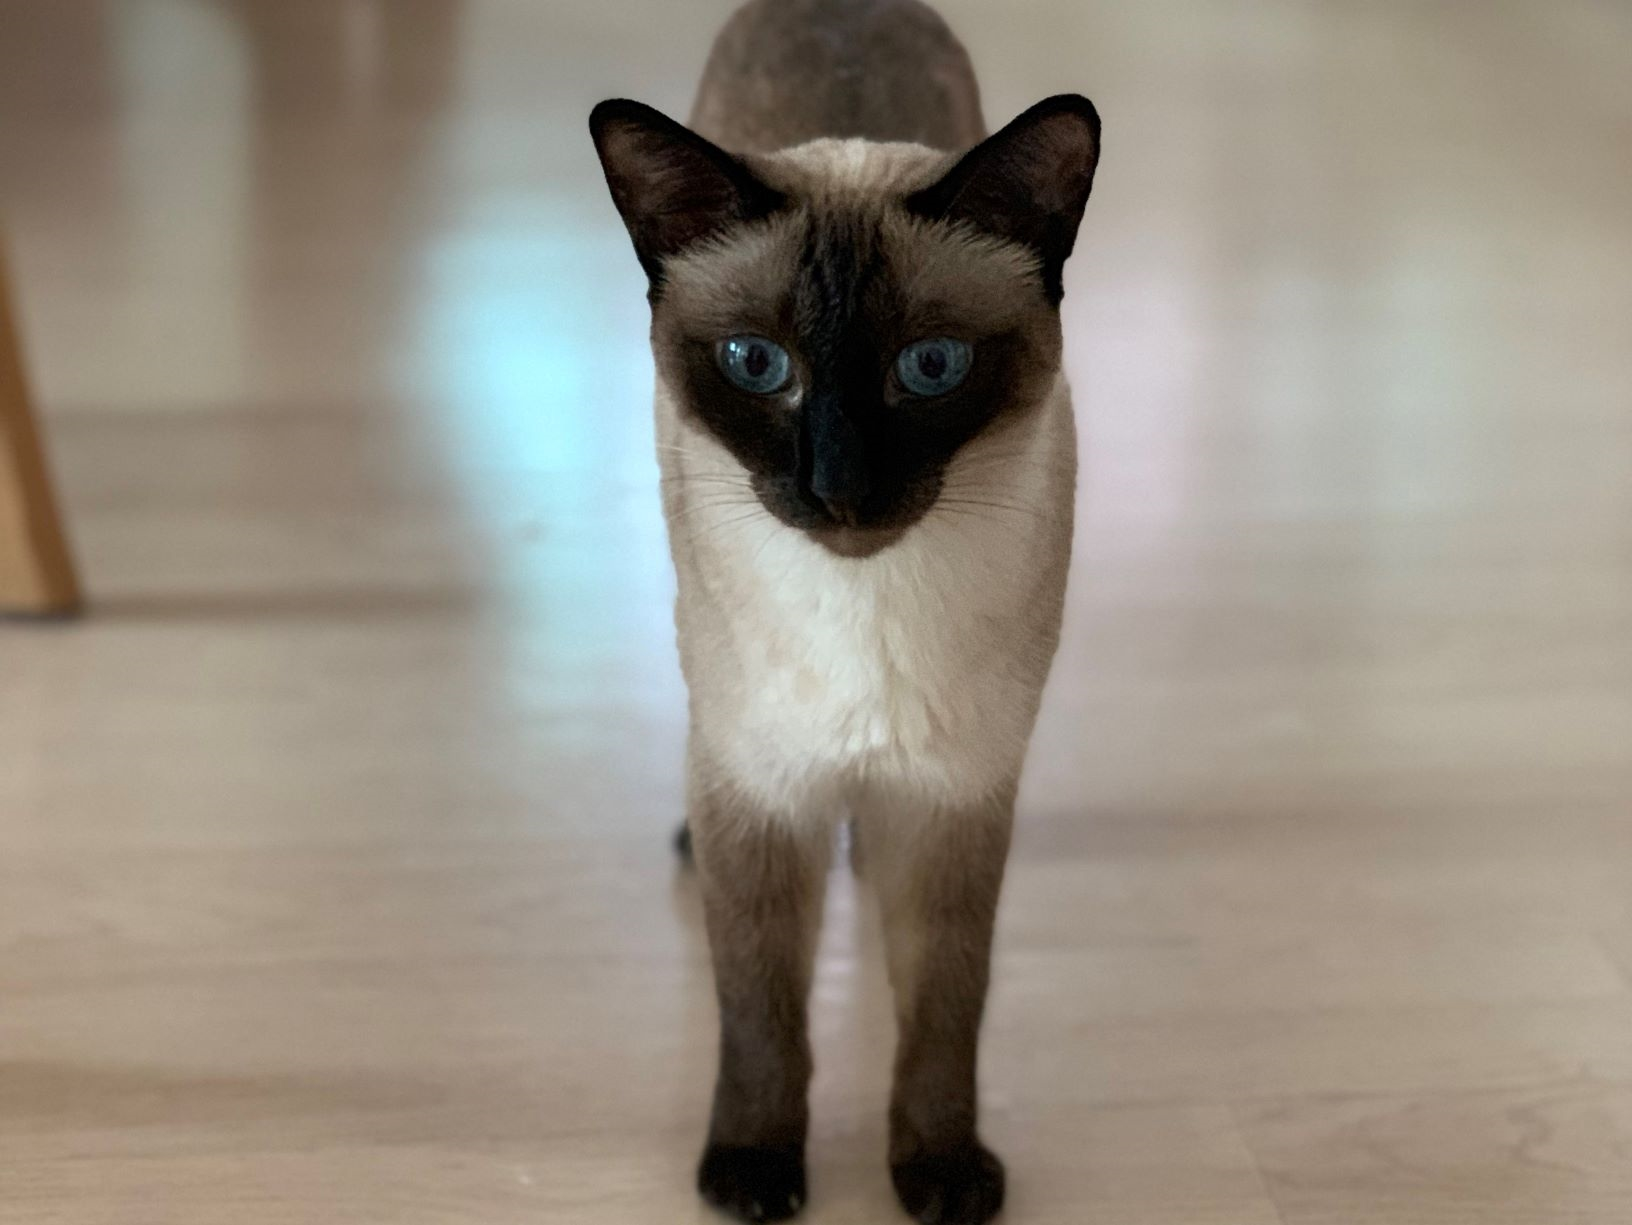
\includegraphics[width=.4\textwidth]{cat.jpg}
\caption{고양이 사진}
\label{fig:cat}
\end{figure}

표의 경우, \textbackslash{table}\와 \textbackslash{tabular}\를 사용하여 원하는 표를 생성할 수 있습니다.
그림의 경우, \textbackslash{figure}\를 사용하여 그림을 삽입할 수 있습니다.
캡션은 그림은 하단에, 표는 상단에 위치하도록 합니다.
그림이나 표를 참조할 경우, \textbackslash{ref}를 사용하여 참조할 수 있습니다. 그림 \ref{fig:cat} 및 표 \ref{tab:data_stats}\으로 표시합니다\footnote{\url{https://en.wikibooks.org/wiki/LaTeX/Floats,_Figures_and_Captions}에서 그림 및 표 작성법에 대해 알아볼 수 있다.}.
참조 번호는 논문에서 언급된 순서대로 자동 부착됩니다.

\subsubsection{조사 자동 부착}
\begin{figure}[t]
\centering
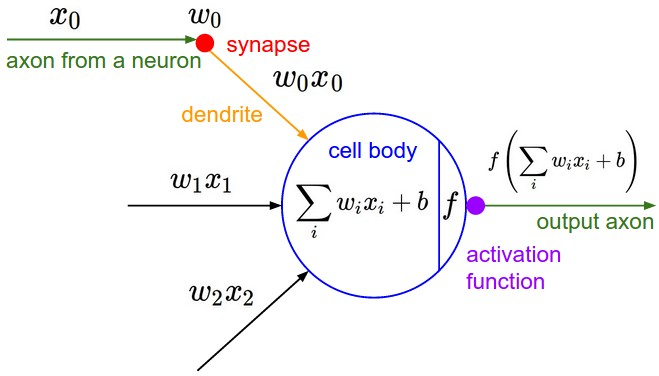
\includegraphics[width=.4\textwidth]{neuron.jpg}
\caption{Neuron Model (cs231n 강의노트 참조)}
\label{fig:neuron}
\end{figure}

한국어는 참조 번호에 따라 조사를 달리 사용합니다. 예를 들어, 그림의 참조 번호가 1이면 
조사 '을', 참조 번호가 2이면 조사 '를'을 사용해야 합니다.
(그림 1\textbf{을}..., 그림 2\textbf{를}...)
%그림 1\textbf{을}, 참조 번호가 2이면 그림 2\textbf{를} 사용하여야 합니다. 
표나 그림을 중간에 추가해야하는 상황이 발생된다면 조사 또한 일일이 수정해야하는 번거로움이 존재하게 됩니다.

본 파일은 자동조사를 통해, 참조 번호에 따라 자동으로 선택할 수 있는 방법을 제공합니다. `은/는'의 경우, `\textbackslash{은}'으로만 표기를 하면 자동으로 `은/는' 중 적합한 조사를 선택합니다. 그림 \ref{fig:cat}\은 고양이 그림이며, 그림 \ref{fig:neuron}\은 뉴런 모델 그림입니다\footnote{hclt.tex에서 이 부분을 직접 참고하시기 바랍니다.}. 자동입력을 지원하는 조사는 총 12가지이며, 아래와 같습니다.

\textbackslash{이}, \textbackslash{가}, \textbackslash{을}, \textbackslash{를}, \textbackslash{와}, \textbackslash{과}, \textbackslash{로}, \textbackslash{으로}, \textbackslash{은}, \textbackslash{는}, \textbackslash{라}, \textbackslash{이라}

자세한 내용은 \url{http://tug.ctan.org/language/korean/kotex-utf/doc/kotexdoc.pdf}파일에서 `5.3.10 자동조사 명령'을 참고하기 바랍니다

\section{참고문헌 작성법}
본 논문에서 사용하는 참고문헌 작성 스타일은 IEEE에서 제공하는 `IEEEtran.bst' 파일을 수정하여 만들었습니다.
첨부된 `IEEEtran.bst'파일을 참고문헌 작성 스타일로 사용하면 (\textbackslash{bibliographystyle\{IEEEtran\}}), 
한글 파일 양식에서 언급한 저자, 제목, 학술지명, 권, 호, 쪽수, 발행년도 순으로 자동 기술됩니다.
\textbackslash{cite}를 사용하여 참고문헌의 번호를 참조할 수 있습니다. 
예를 들어, 색인어 구축을 위해 한국어 형태소 분석기~\cite{kang:hclt94}를 활용한 연구가 있었다~\cite{choi:jiise96}.
여러 연구를 참조할 경우, 콤마를 사용하여 참조할 연구들을 나열하면 됩니다~\cite{kang:BOOK2002,mani:BOOK1999,bengio:jmlr03,Burl:ECCV1998}.

\section{결론}
이 부분은 결론을 적는 부분입니다. 이 부분은 결론을 적는 부분입니다. 이 부분은 결론을 적는 부분입니다.

\section*{감사의 글}
심사용 논문에는 감사의 글을 표기하지 않습니다. 심사용으로 논문 제출시 감사의 글을 주석처리 하기 바랍니다.

\bibliographystyle{IEEEtran}
\bibliography{refer}

\end{document}
